\chapter{Pricing: Learning the Best Price}

In this chapter we are going to focus our attention on the pricing and on the optimal price, that we can propose to our customers, to maximize the total revenue.

In common scenarios, in which there is a seller that has to sell products, the retail price is fixed without exploiting information from the buyers.\\
Sometimes, in physical markets, the customers have the possibility to negotiate and a skillful seller can maximize his revenue keeping the price as high as possible. This is a common practice, but experience is needed, to understand the limit of the buyers, and moreover it requires time, loosing the possibility to serve other clients.\\
In e-commerce scenarios, we can do better exploiting information from the users, from the big data and from the software automation.
In particular, given the assignments~\ref{assPart4}, we are going to design an algorithm being able to learn the optimal price for our product, to maximize the total revenue.

In the following steps, we are going to:
\begin{itemize}
	\item define the demand curves of the users;
	\item describe the environment setup;
	\item explain the algorithm that has been chosen; and
	\item comment the results obtained in the end of the campaign.
\end{itemize}


\section{Demand Curves}

In the economic literature is defined the concept of \textbf{demand curve}.
It is a function that maps the price to a certain probability. In other words, given a price, the function returns the probability that the product will be sold. Therefore, if we plot the demand curve, we'll obtain on the x-axis the admissible prices and on the y-axis the probability (between $0$ and $1$).

In our simulated scenario, we defined three classes of users with the corresponding demand curves. The shapes of the curves are motivated by the intrinsic behaviors of the classes:
\begin{itemize}
	\item \textit{Elegant}: they are rich, thus they will buy the product with high probability whatever is the proposed price;
	\item \textit{Casual}: they are students, thus they are able to buy the product only if the price is relatively low; and
	\item \textit{Sports}: they are workers, but without a particular interest on the shoes, therefore the price is relatively irrelevant and the probability is low.
\end{itemize}

In figure \ref{demandCurvesFig} there are the curves designed following the above descriptions.
\footnote{A tool as been implemented to draw the curves manually. It requires few points and it performs polynomial regression to augment the sampling definition. It can be found in the attached code.}

In the same figure, the \textit{aggregate} curve has been reported (colored in \textit{orange}), it represents the mean between the other curves. (It will be useful in the next subsections.)\\
Moreover, points representing the theoretical optimum are reported. The area below them is maximum w.r.t. the curves.

\begin{figure}[H]
	\centering
	%\captionsetup{justification=centering,margin=1cm}

	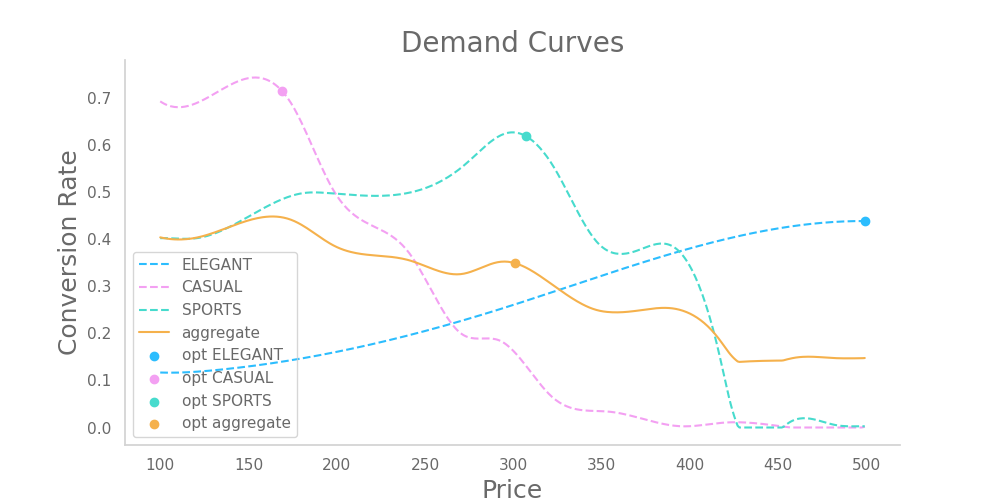
\includegraphics[width=1.0\textwidth]{images/demand_curves.png}
	\caption{\textbf{Demand Curves}.\\
		They are used to model the probability (\textit{conversion rate}) that a certain class, of customers, will buy or not the product w.r.t. a proposed price.\\
		The dashed lines represent the demand curves of the corresponding classes:
		\textit{blue} for the \textit{Elegant} class;
		\textit{pink} for the \textit{Casual} class; and
		\textit{light green} for the \textit{Sports} class.\\
		The \textit{orange} curve is the mean between the others and it is used to study the \textit{aggregate} model.\\
		The points are displayed to show the optimal price w.r.t. the conversion rate: the area below them is maximum.}
		\label{demandCurvesFig}
\end{figure}

\section{Environment}

In our implementation, the environment is a black box from the point of view of the learning algorithm.
It is used to iterate over the days, for the entire duration of the campaign.
It schedules the time and the number of users reaching our theoretic website.

Every user is randomly taken from the three classes and the class is not communicated to the learner. The environment, knowing the original class of the users, computes the optimal revenue and returns the effective reward obtained by the learner.

How the learner will handle these information will be explained in the next subsections.

\section{Learner Algorithm Selection}

This context of application can be solved in different ways, but the most common choice is to use a \textit{multi-armed bandit (MAB)} algorithm.

We mainly tested two algorithms:
\begin{itemize}
	\item \textbf{Thompson Sampling (TS)} algorithm; and
	\item \textbf{Thompson Sampling with Sliding Window (SWTS)} algorithm.
\end{itemize}

We tested both the algorithms during the implementation phase, but since the SWTS is more sensible to the window size, and finding a good one requires a lot of testing, we kept the TS as final choice.\\
This decision has been motivated by the fact that there aren't abrupt phases, thus there is no reason to "forgot the past" as done by SWTS.


\section{Experiments}

Summarizing, we have to learn the best price to propose, to the users, to maximize the total revenue.\\
We have discussed about the environment, that generates incoming users and allows us to iterate over the days of the campaign, and finally, we presented the learner adopted.\\
At this point we can explain how the tests have been initialized.

The experiments has been configured in two ways:
\begin{itemize}
	\item keeping a fixed daily price: we pulled an arm only for the first user of the day; for the other users we proposed always the same price. This means that for the entire day we pull and update always the same arm of the TS;
	\item one price for each user: maybe, this is an unpractical option in a real world scenario, but it allows to obtain a total revenue outperforming the previous configuration.
\end{itemize}

In the end of the tests, the figure \ref{regret4Fig} reports the obtained regrets. The sub figure \textit{(a)} for the first configuration and the sub figure \textit{(b)} for the second.

We plotted two regrets computed with two different optimal revenues.
The regret called \textbf{Mean Regret of the Aggregate Model} has been computed using, as optimal, the optimal point taken from the aggregate model. This is an optimistic regret because it doesn't take into consideration the information about the specific class of the users. In other words, the learner and the clairvoyant algorithm don't know the class of the customers.

The learner is learning the aggregate model, thus this comparison seams fair, but since the clairvoyant knows the original class of the users, we introduced the so called \textbf{Mean Regret of the True Evaluation}. Obviously, from the point of view of the learner, this is a pessimistic computation since it is unable to infer more information from the input data.

Anyway, these two ways, to compute the regrets, will be useful in the next chapter, since the learner will be able to infer more information from the data, creating contexts to exploit a finer profiling.
You will notice how the two regrets will be pushed down and the regret on the True Evaluation will be more similar to the regret of the Aggregate Model obtained here, proving that a finer profiling improves drastically the performances.


\begin{figure}[!htb]
	\centering
	%\captionsetup{justification=centering,margin=1cm}
	
	\begin{subfigure}[!H]{0.8\textwidth}
		\centering
		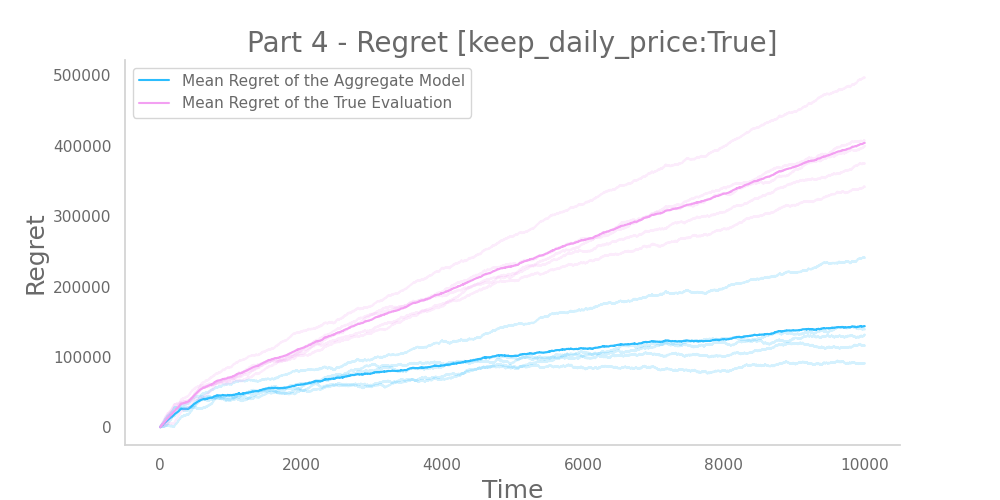
\includegraphics[width=\textwidth]{images/part4_keep-daily-priceTrue.png}
		\caption{Regret obtained proposing to the customers the same price for the entire day.}
	\end{subfigure}
	%\hfill
	\begin{subfigure}[!H]{0.8\textwidth}
		\centering
		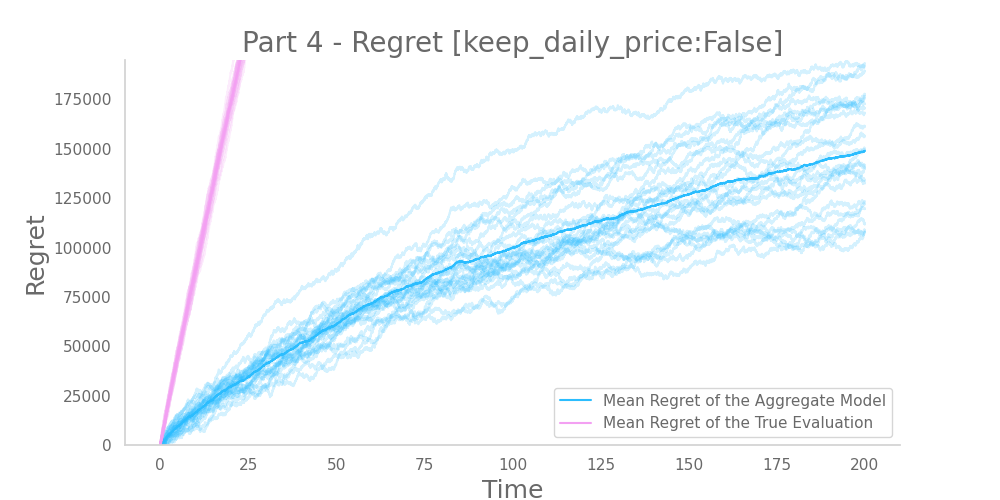
\includegraphics[width=\textwidth]{images/part4_keep-daily-priceFalse.png}
		\caption{Regret obtained proposing to the customers different prices for each visit. This method achieves better performances since the learner collects more data during the campaign.}
	\end{subfigure}

	\caption{Comparison between the regrets obtained during the campaign.\\
			The \textbf{Mean Regret of the Aggregate Model} (colored in \textit{blue}) is the regret computed keeping, as optimal, the area under the optimal point of the aggregate curve~\ref{demandCurvesFig}. In other words, both the learner and the clairvoyant don't know the class of the customers. This is an optimistic measure of the regret.\\
			The \textbf{Mean Regret of the True Evaluation} (colored in \textit{pink}) is the regret obtained computing the optimal value exploiting the original class of the customers.}
	\label{regret4Fig}
\end{figure}